
\subsection{Cardinal}

\noindent Le \textit{cardinal} est le nombre de valeurs contenues dans une distribution.

\begin{center}
\begin{equation*}
\text{Nombre de Valeurs} = \text{cardinal de la distribution} = \text{\textit{card}}(L) = |L|
\end{equation*}
\end{center}


\bigskip


\subsection{\'Etendue}

\noindent L'\textit{étendue} est la différence entre la plus grande valeur de la distribution et la plus petite valeur de la distribution.

\begin{center} % \text{étendue} = \text{Valeur}_{\text{\textit{max}}} - \text{Valeur}_{\text{\textit{min}}}
\begin{equation*}
\text{étendue} = E = \text{\textit{max}}(L) - \text{\textit{min}}(L)
\end{equation*}
\end{center}


\bigskip


\subsection{Moyenne}

\noindent La \textit{moyenne arithmétique}, communément appelée \textit{moyenne}, est la somme de tous les éléments de la distribution divisée par le cardinal.

\begin{center} % \text{moyenne} = \frac{\sum_{n=1}^{\text{Nb Valeurs}} \text{Valeur}_{i}}{\text{Nb Valeurs}}
\[
\text{moyenne} = \mu = \bar{L} = \frac{\displaystyle \sum L_{i}}{|L|}
\]
\end{center}

% DistrNbValues = 10
% moyenne = 0
% for (x in range(0, DistrNbValues)):
%   valeur = int(random.random() * 100)
%   moyenne += valeur
% moyenne = moyenne / DistrNbValues


\bigskip


\subsection{Médiane}

\noindent La \textit{médiane} est la valeur centrale d'une distribution triée.

\begin{itemize}
\item En cas de quantité impaire de valeurs, on prend la valeur à la position $ \frac{n + 1}{2} $.
\item En cas de quantité paire de valeurs, on prend la moyenne des deux valeurs centrales.
\end{itemize}

\begin{center} % \text{médiane} = \text{Valeur}_{\frac{i}{\text{Nb Valeurs}}}
\begin{equation*}
\text{médiane} = L_{\frac{|L|}{2}}
\end{equation*}
\end{center}

\bigskip

\noindent Par exemple pour la distribution suivante : 4 5 6

\noindent La médiane sera de $ 5 $, car $ \frac{3 + 1}{2} = 2 $ et $ 5 $ et le deuxième nombre de la distribution.

\bigskip

\noindent Par exemple pour la distribution suivante : 1 2 3 4

\noindent La médiane sera de $ 2,5 $, car $ 2 $ et $ 3 $ sont les valeurs centrales et $ \mu(2 ; 3) = 2,5 $.

\bigskip

\noindent \textbf{\textit{Attention : n'oubliez pas que Python compte depuis 0 pour la position dans les listes.}}

% import math
% median_pos = int(math.floor(DistrNbValues / 2))
% sorted_distr = MyDistribution.copy()
% sorted_distr.sort()
% median = sorted_distr[median_pos]


\bigskip


\subsection{Quartiles et \'Ecart interquartiles}

\subsubsection{Quartiles}

\noindent L'\textit{écart interquartile} est basé sur la différence entre des \textit{quartiles}.
L'idée des quartiles est de diviser la distribution en $ 4 $ parties, chaque quartile étant un séparateur, et d'observer l'écart entre certains séparateurs pour mesurer la dispersion des valeurs.

\bigskip

\begin{itemize}
\item le quartile 0 ($Q_{0}$) est la valeur la plus petite de la distribution
\item le $ 1^{er} $ quartile ($Q_{1}$) sépare les $ 25\% $ premières valeurs de la distribution des autres
\item le $ 2^{\grave{e}me} $ quartile ($Q_{2}$) sépare les $ 50\% $ premières valeurs de la distribution des autres
\item le $ 3^{\grave{e}me} $ quartile ($Q_{3}$) sépare les $ 75\% $ premières valeurs de la distribution des autres
\item le quartile 4 ($Q_{4}$) est la valeur la plus élevée de la distribution
\end{itemize}

\bigskip

\noindent Plus visuellement, la distribution triée est séparée ainsi :

\begin{center}
$ Q_{0} $ ... (partie 1) ... $ Q_{1} $ ... (partie 2) ... $ Q_{2} $ ... (partie 3) ... $ Q_{3} $ ... (partie 4) ... $ Q_{4} $
\end{center}

\bigskip

\noindent Dans le cas dit \textit{discret} (c'est-à-dire non continu : on peut dénombrer les valeurs que l'on étudie), il n'existe pas une seule méthode universellement acceptée...
Vous implémenterez donc celle de Wikipédia (en français au 20 août 2023) décrite par la suite :
Il suffit de calculer le \textit{rang} des valeurs, c'est-à-dire leur position dans la distribution triée par ordre croissant.
Un quartile dans le cas discret est donc simplement une valeur à une position précise dans la distribution triée.

\bigskip

\noindent Pour une distribution contenant $ n $ valeurs, on calcule les rangs ainsi :

\begin{itemize}
\item le quartile 0 ($Q_{0}$) est donc au rang $ 1 $
\item le $ 1^{er} $ quartile ($Q_{1}$) est au rang $ (n + 3) / 4 $
\item le $ 2^{\grave{e}me} $ quartile ($Q_{2}$) est au rang $ (n + 1) / 2 $ \textit{(il s'agit de la médiane)}
\item le $ 3^{\grave{e}me} $ quartile ($Q_{3}$) est au rang $ (3n + 1) / 4 $
\item le quartile 4 ($Q_{4}$) est donc au rang $ n $
\end{itemize}

\bigskip

\noindent Testons sur la distribution : $ 10 \; 20 \; 30 \; 40 \; 50 \; 60 \; 70 \; 80 \; 90 $

\begin{itemize}
\item $ Q_{0} = L_{1} = 10 $
\item $ Q_{1} = L_{3} = 30 $
\item $ Q_{2} = L_{5} = 50 $
\item $ Q_{3} = L_{7} = 70 $
\item $ Q_{4} = L_{9} = 90 $
\end{itemize}

\bigskip

\noindent La première partie contient donc les valeurs de $ 10 \; 20 \; 30 $, la deuxième partie les valeurs de $ 30 \; 40 \; 50 $, la troisième partie les valeurs $ 50 \; 60 \; 70 $, et la quatrième partie les valeurs $ 70 \; 80 \; 90 $.

\bigskip

\noindent Testons maintenant sur la distribution : $ 10 \; 20 \; 30 \; 40 \; 50 \; 60 \; 70 \; 80 $

\begin{itemize}
\item $ Q_{0} = L_{1} = 10 $
\item $ Q_{1} = L_{2,75} = ?? $
\item $ Q_{2} = L_{4,5}  = ?? $
\item $ Q_{3} = L_{6,25} = ?? $
\item $ Q_{4} = L_{8} = 80 $
\end{itemize}

\bigskip

%Si on ne tombe pas sur un rang précis, il est normalement nécessaire de calculer un poids entre la valeur au dessus et la valeur au dessous.
%Mais pour simplifier notre cas, utilisons le rang inférieur (avec \TTBF{math.floor}).
%Si on ne tombe pas sur un entier pour le rang, on effectue la moyenne entre le rang inférieur (avec \TTBF{math.floor}) et le rang supérieur (avec \TTBF{math.ceil}) exactement comme lors du calcul de la médiane.
\noindent Si on ne tombe pas sur un entier pour le rang, on effectue la moyenne entre le rang inférieur et le rang supérieur en affectant des poids :

\bigskip

\begin{itemize}
\item si le reste après la virgule est à $ 0,25 $ : on affecte le poids $ 3 $ au rang inférieur, et le poids $ 1 $ au rang supérieur
\end{itemize}
\vspace*{-1cm}
\begin{center}
\[ \scalebox{1.15}{$\displaystyle Q_{X} = \frac{3 * L_{n - 1} \; + \; 1 * L_{n + 1}}{3 \; + \; 1} $} \]
\end{center}

\begin{itemize}
\item si le reste après la virgule est à $ 0,5 $ : on affecte le poids $ 1 $ au rang inférieur, et le poids $ 1 $ au rang supérieur (cela revient à la moyenne des deux)
\end{itemize}
\vspace*{-1cm}
\begin{center}
\[ \scalebox{1.15}{$\displaystyle Q_{X} = \frac{1 * L_{n - 1} \; + \; 1 * L_{n + 1}}{1 \; + \; 1} $} \]
\end{center}

\begin{itemize}
\item si le reste après la virgule est à $ 0,75 $ : on affecte le poids $ 1 $ au rang inférieur, et le poids $ 3 $ au rang supérieur
\end{itemize}
\vspace*{-1cm}
\begin{center}
\[ \scalebox{1.15}{$\displaystyle Q_{X} = \frac{1 * L_{n - 1} \; + \; 3 * L_{n + 1}}{1 \; + \; 3} $} \]
\end{center}

\bigskip

\noindent Reprenons la distribution : $ 10 \; 20 \; 30 \; 40 \; 50 \; 60 \; 70 \; 80 $

\begin{flalign*}
& \scalebox{1.15}{$Q_{0} = L_{1} = 10$} \\
& \scalebox{1.15}{$Q_{1} = L_{2,75} = \frac{1 * L_{2} \; + \; 3 * L_{3}}{1 \; + \; 3} = \frac{1 * 20 + 3 * 30}{1 + 3} = \frac{110}{4} = 27,5$} \\
& \scalebox{1.15}{$Q_{2} = L_{4,5}  = \frac{1 * L_{4} \; + \; 1 * L_{5}}{1 \; + \; 1} = \frac{1 * 40 + 1 * 50}{1 + 1} = \frac{90}{2} = 45$} \\
& \scalebox{1.15}{$Q_{3} = L_{6,25} = \frac{3 * L_{6} \; + \; 1 * L_{7}}{3 \; + \; 1} = \frac{3 * 60 + 1 * 70}{3 + 1} = \frac{250}{4} = 62,5$} \\
& \scalebox{1.15}{$Q_{4} = L_{8} = 80$} \\
\end{flalign*}


% Q0 = 1
% Q1 = (DistrNbValues + 3) / 4
% Q2 = DistrNbValues / 2
% Q3 = ((3 * DistrNbValues) + 1) / 4
% Q4 = DistrNbValues

\bigskip


\subsubsection{\'Ecart interquartile}

\noindent L'\textit{écart interquartile} ou \textit{étendue interquartile} (ou \textit{interquartile range} en anglais et son acronyme \textit{IQR}) est simplement la différence entre le quartile 3 et le quartile 1.

\begin{center} % \text{étendue} = \text{Valeur}_{\text{\textit{max}}} - \text{Valeur}_{\text{\textit{min}}}
\begin{equation*}
\text{écart interquartile} = EI = Q_{3} - Q_{1}
\end{equation*}
\end{center}

% EI = Q3 - Q1


\bigskip


\subsection{Variance}

\noindent La \textit{variance} permet de mesurer la dispersion des valeurs de la distribution par rapport à la moyenne.
L'interprétation est simple : une variance élevée indique que les nombres de la distribution sont éloignés de la moyenne ($ 1 $ et $ 99 $ par rapport à $ 50 $), une variance faible indique que les nombres de la distribution sont proches de la moyenne ($ 42 $ et $ 58 $ par rapport à $ 50 $).
Ici, nous implémenterons la variance d'une population complète, et non pas juste d'un échantillon.

% \frac{\displaystyle (\sum E_{i}^{2}) - \frac{\displaystyle (\sum E_{i})^{2}}
%                                             {\displaystyle \text{Nb Valeurs}}}
%      {\displaystyle \text{Nb Valeurs}}

\begin{center}
\begin{equation*}
\text{variance} = \sigma^{2} = Var(L) = \frac{1}{|L|} \sum (L_{i} - \bar{L})^{2}
\end{equation*}
\end{center}

\bigskip

\noindent Ce calcul peut paraître rebutant, mais il est très simple lorsque l'on regarde de plus près chaque partie de l'expression :

\medskip

\begin{itemize}
\item[$\bullet$] $ (L_{i} - \bar{L}) $ correspond à la différence entre chaque élément de la distribution et la moyenne de la distribution.

\item[$\bullet$] $ (L_{i} - \bar{L})^{2} $ correspond au carré de la différence entre chaque élément de la distribution et la moyenne de la distribution.

\item[$\bullet$] $ \sum (L_{i} - \bar{L})^{2} $ correspond à la somme des carrés précédemment décrits. Il s'agit donc de faire une boucle effectuant les traitements précédemment décrits, pour ajouter le résultat à une variable initialisée à $ 0 $ juste avant la boucle.

\item[$\bullet$] $ \frac{1}{|L|} \sum (L_{i} - \bar{L})^{2} $ correspond à la division par le nombre d'éléments de la distribution du total de la somme précédente.
\end{itemize}

%def Variance1(MyDistribution):
%  DistrNbValues = length(MyDistribution)
%  Moyenne = 0
%  for x in MyDistribution:
%    Moyenne = Moyenne + x
%  Moyenne = Moyenne / DistrNbValues
%  tmp = 0
%  for x in MyDistribution:
%    tmp = tmp + ((x - Moyenne) ** 2)
%  variance = tmp / DistrNbValues
%  return (variance)

\bigskip

\noindent En développant le calcul, on peut arriver à une formule beaucoup plus adaptée au développement, surtout avec des distributions extrêmement grandes (c'est-à-dire des distributions sur lesquelles il coûterait très/trop cher de passer plusieurs fois pour calculer tout d'abord la \textit{moyenne}, et seulement ensuite la différence de chaque élément avec la moyenne), ou lorsque les valeurs arrivent au fur et à mesure sans savoir précisément quand la distribution s'arrêtera (et que l'on souhaite un aperçu des statistiques en temps réel) :

\begin{center}
\begin{equation*}
\text{variance} = \sigma^{2} = Var(L) = \frac{1}{|L|} \sum (L_{i} - \bar{L})^{2} = \left( \frac{1}{|L|} \sum L_{i}^{2} \right) - \bar{L}^{2}
\end{equation*}
\end{center}

\bigskip

\noindent Analysons cette deuxième formule pour comprendre son intérêt en tant que développeur :

\medskip

\begin{itemize}
\item[$\bullet$] $ L_{i}^{2} $ correspond à la mise au carré de chaque élément de la distribution.

\item[$\bullet$] $ \sum L_{i}^{2} $ correspond à la somme de tous les éléments de la distribution mis au carré individuellement, c'est-à-dire d'itérer sur chaque élément, en faire son propre carré, puis d'ajouter ce résultat à une variable mise à $ 0 $ juste avant la boucle.

\item[$\bullet$] $ \frac{1}{|L|} \sum L_{i}^{2} $ correspond à la division de la somme précédente par le nombre d'éléments de la distribution.

\item[$\bullet$] $ ( \frac{1}{|L|} \sum L_{i}^{2} ) - \bar{L}^{2} $ correspond à la différence entre la division précédente, et la moyenne de la distribution mise au carré.
\end{itemize}

\noindent Cette deuxième formule est en réalité bien plus efficace dans un contexte séquentiel (c'est-à-dire lorsque chaque opération est effectuée l'une après l'autre), car nous pouvons faire une somme de tous les éléments qui arrivent et une somme de chacun de leur carré, et seulement lorsque tous les nombres ont été analysés, nous pouvons en déduire la moyenne et la soustraire.
Chaque élément n'aura été lu qu'une seule et unique fois lorsqu'il a été généré, et nous avons fait évolué deux variables distinctes à côté : une somme simple (pour produire la moyenne), et une somme des carrés.

%sumelt = 0
%sumsqelt = 0
%DistrNbValues = N
%
%def Generation(N):
%  for x in range(0, N):
%    elt = random.randint()
%    sumelt = sumelt + elt
%    sumsqelt = sumsqelt + (elt ** 2)
%  ...
%
%def Variance2(MyDistribution):
%  variance = (sumsqelt - ((sumelt ** 2) / DistrNbValues) / DistrNbValues)
%  return (variance)


\bigskip


\subsection{\'Ecart type}

\noindent L'\textit{écart type} (ou \textit{standard deviation} en anglais) permet de mesurer la dispersion d'une distribution.
Plus la mesure est élevée, plus la distribution contient des valeurs éloignées ($ 3 $ et $ 90 $), et plus la mesure est faible, plus la distribution contient des valeurs proches ($ 42 $ et $ 46 $).
On peut comparer les écarts types de distributions issues de mêmes choses (par exemple, les écarts types de plusieurs classes composées d'étudiants).
Ici, nous implémenterons l'écart type d'une population complète, et non pas juste d'un échantillon.

\begin{center}
\begin{equation*}
\text{écart type} = \sigma = \sqrt{Var(L)}
\end{equation*}
\end{center}

% import math
% stddev = math.sqrt(Variance1(MyDistribution))


\bigskip


\subsection{Coefficient de variation/\'Ecart type relatif}

\noindent Le \textit{coefficient de variation} ou \textit{écart type relatif} (ou \textit{relative standard deviation} en anglais et son acronyme \textit{RSD}) permet de mesurer la dispersion d'une distribution autour de la moyenne en générant un pourcentage indépendant des objets étudiés par la distribution.
Plus le pourcentage est faible, plus la distribution est concentrée autour de sa moyenne, plus le pourcentage est élevé, plus la distribution est étalée loin de sa moyenne.
Cependant, l'écart type relatif ne fonctionne pas lorsque la moyenne est proche de $ 0 $ : celui-ci va tendre vers l'infini (donc dépasser les $ 100\% $) et sera très sensible aux variations.
Ici, nous implémenterons l'écart type relatif d'une population complète, et non pas juste d'un échantillon.

\begin{center}
\begin{equation*}
\text{coefficient de variation} = c_{v} = \frac{\sigma}{\mu} = \frac{\sqrt{Var(L)}}{\bar{L}}
\end{equation*}
\end{center}

% import math
% stddev = math.sqrt(Variance1(MyDistribution))
% RSD = stddev / mean(MyDistribution)


\bigskip


\subsection{Coefficient de Gini}

\noindent Le \textit{coefficient de Gini} est un indice particulièrement utilisé dans le monde économique et social.
Ce coefficient a été constitué pour mesurer les inégalités de revenus au sein d'une population, mais il permet plus généralement de mesurer l'inégalité de répartition d'une variable (donc son interprétation s'approche des mesures de dispersion).
Le coefficient de Gini calcule une valeur entre $ 0 $ (égalité parfaite entre toutes les valeurs de la distribution) et $ 1 $ (inégalité totale/une seule valeur est positive, et toutes les autres sont nulles).

\noindent Le calcul théorique de ce coefficient peut paraitre très rebutant à cause des termes employés, et pourtant, il est très facile à comprendre.
De plus, le calcul pratique dans le cas discret (pour rappel : non continu/on peut dénombrer les valeurs de la distribution), n'est pas complexe.

\bigskip

\noindent Le coefficient de Gini est défini comme le double de l'aire entre la courbe de Lorenz d'une distribution parfaitement égalitaire, et la courbe de Lorenz de la distribution étudiée.

\noindent Qu'est-ce qu'une \textit{courbe de Lorenz} ?
Tout simplement la courbe formée par la somme des éléments triés par ordre croissant d'une distribution.
Plus visuellement, le tracé bleu correspond à la courbe de Lorenz de la distribution $ 5 \; 10 \; 40 \; 5 \; 40 $, et le tracé rouge correspond à la courbe de Lorenz d'une distribution parfaitement égalitaire.

\bigskip

\begin{center}
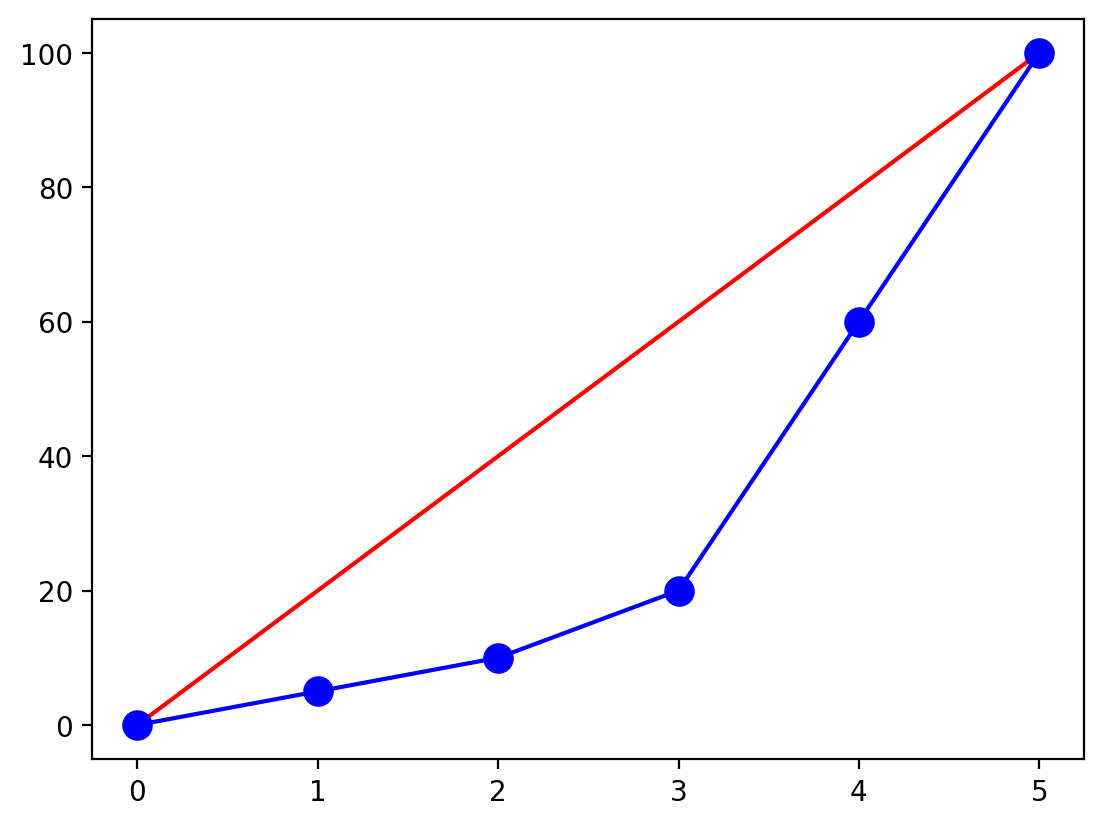
\includegraphics[scale=0.60]{images/exemple_courbe_lorenz_simple.png}
\end{center}

\bigskip

\noindent Encore plus visuellement, une fois la distribution ordonnée, on obtient donc $ 5 \; 5 \; 10 \; 40 \; 40 $.
L'histogramme suivant montre visuellement chaque valeur ajoutée entre les points de la courbe bleue.
Donc, en effectuant la somme des valeurs au fur et à mesure, chaque point de la courbe bleue correspond à $ 5 \; 10 \; 20 \; 60 \; 100 $.

\bigskip

\begin{center}
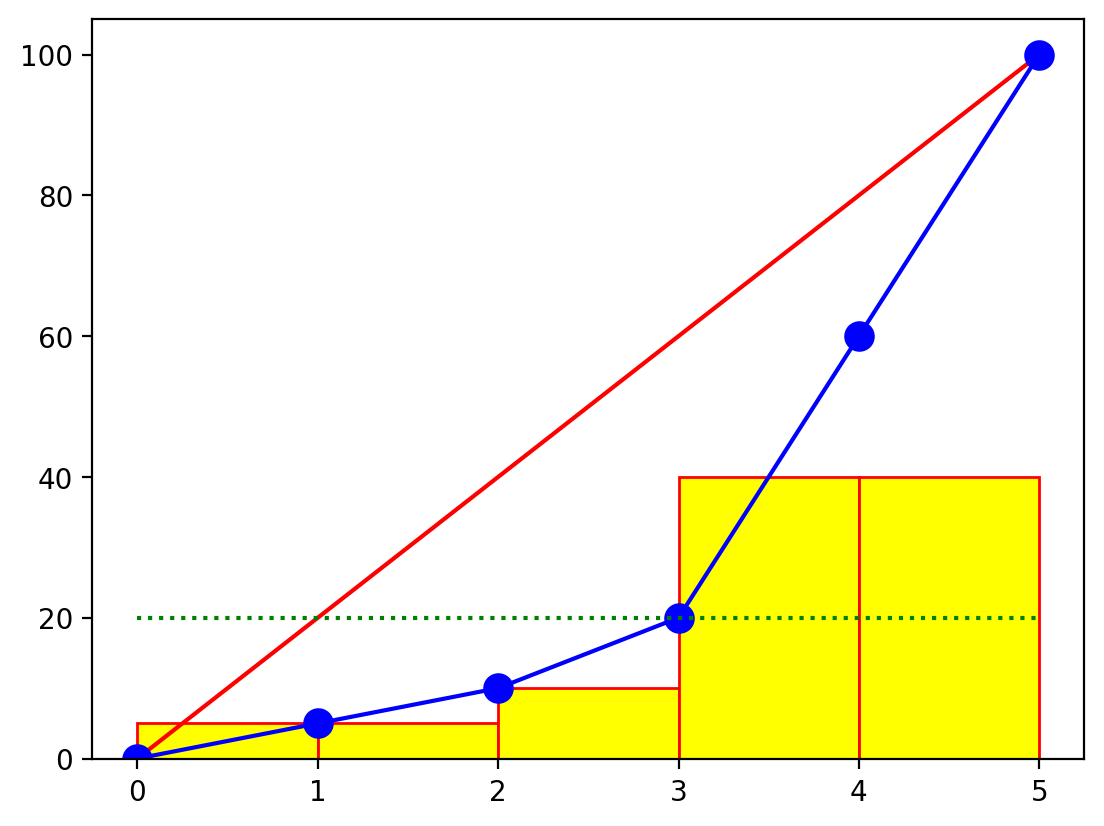
\includegraphics[scale=0.60]{images/exemple_courbe_lorenz-5-5-10-40-40.png}
\end{center}

\bigskip

\noindent Pour rappel, le coefficient de Gini correspond au double de l'aire entre la courbe bleue et la courbe rouge.
Pour bien apprécier visuellement l'écart de cette aire, prenons maintenant deux autres distributions, et comparons l'ensemble des cas :

\begin{itemize}
\item[$\bullet$] $ 0 \; 0 \; 0 \; 10 \; 90 $ (une distribution très inégale) : $ \text{Coeff Gini} = 0,760 $
\item[$\bullet$] $ 5 \; 5 \; 10 \; 40 \; 40 $ (une distribution plutôt inégale) : $ \text{Coeff Gini} = 0,424 $
\item[$\bullet$] $ 10 \; 15 \; 20 \; 25 \; 30 $ (une distribution peu inégale) : $ \text{Coeff Gini} = 0,200 $
\end{itemize}

\bigskip

\noindent Pour bien visualiser ces cas, la moyenne des distributions ($ 20 $) a été tracée en pointillés verts.

\begin{center}
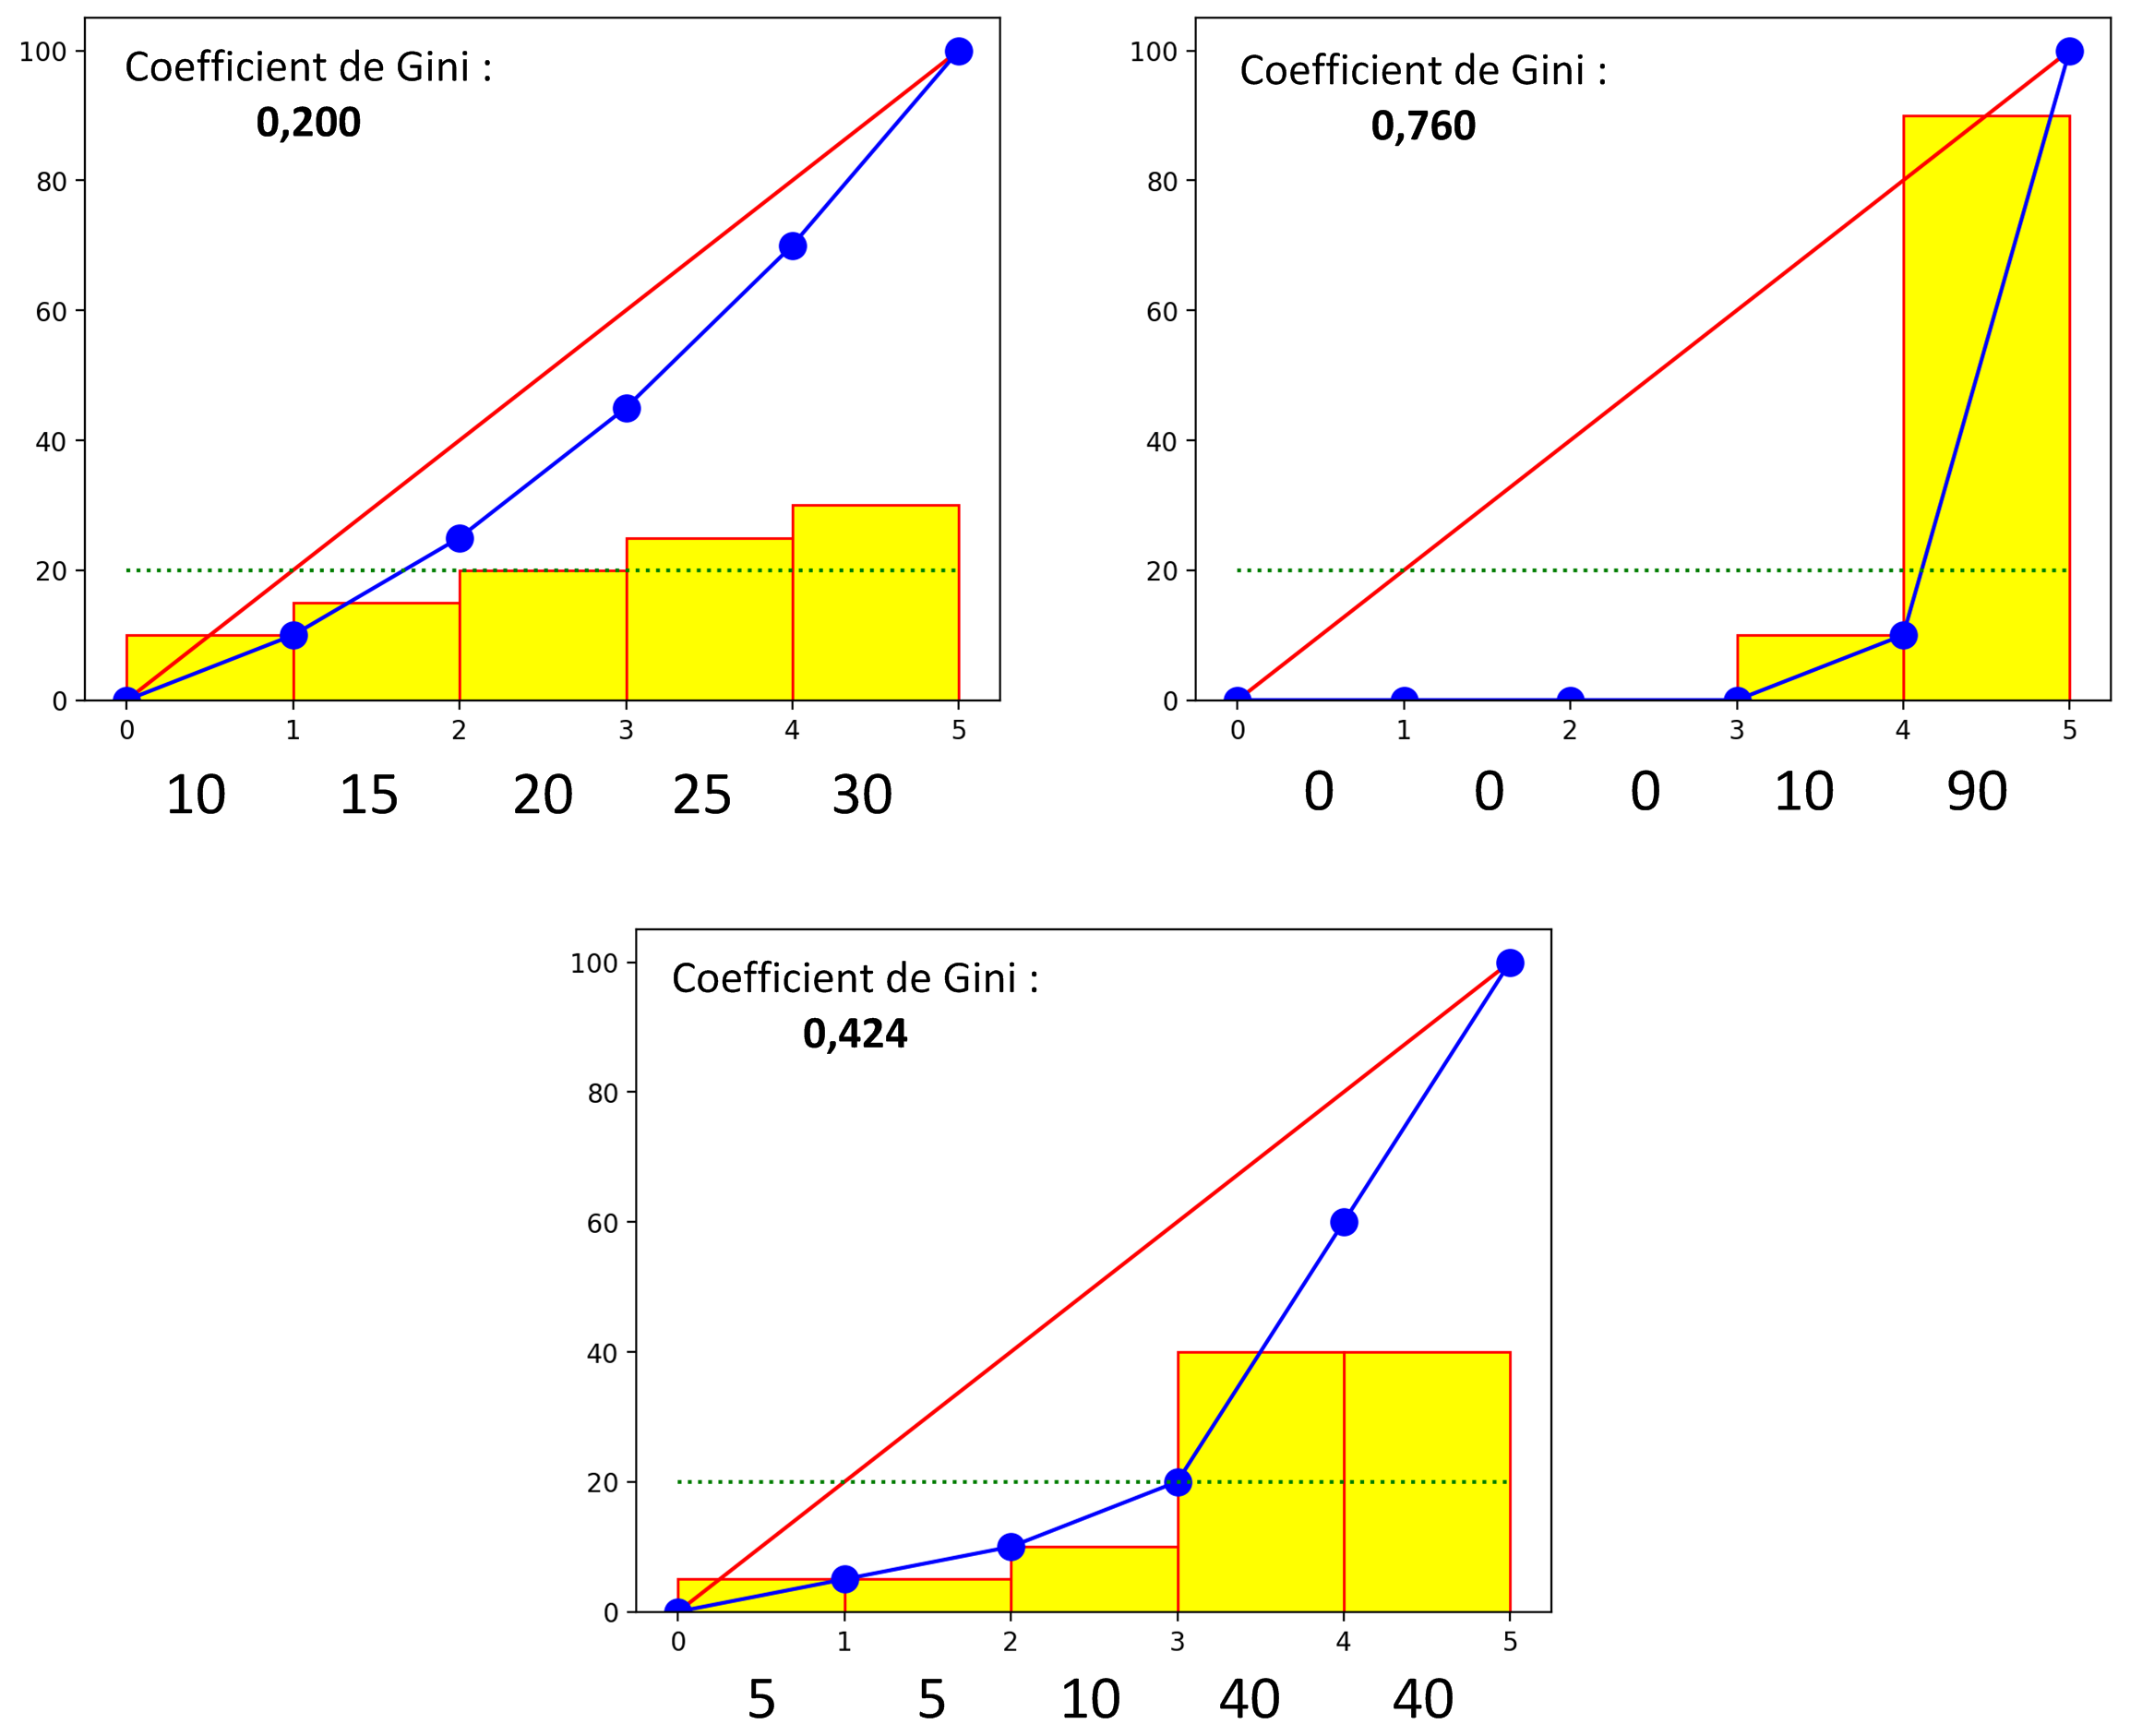
\includegraphics[scale=0.54]{images/exemple_courbes_lorenz.png}
\end{center}

\noindent Comme vous pouvez le constater, le cas peu inégal montre une courbe bleue proche de la courbe rouge, et inversement, le cas très inégal montre une courbe bleue très éloignée de la courbe rouge.
Pour rappel, la moyenne n'est pas un indicateur de dispersion, mais bien un indicateur de tendance centrale ou de position.
Les nombreux indicateurs que vous venez d'implémenter vous permettront donc de mieux interpréter les données dont vous disposerez dans votre carrière, et éventuellement de voir des phénomènes jusque-là peu visibles.

\bigskip

\noindent Reprenons l'implémentation du coefficient de Gini : vous venez de comprendre comment celui-ci est théoriquement construit et interprété.
Mais comment l'implémenter facilement ?

\noindent Deux formules nous intéressent particulièrement, la première est l'équation de Kendal et Stuart.
Dans celle-ci, $ n $ correspond au nombre d'éléments dans la distribution, et $ L_{1} , L_{2} , ... , L_{n} $ correspondent à chaque élément de la distribution.

\begin{center}
\begin{equation*}
G = \frac{ (1 / 2 n^{2}) \, \overset{n}{\underset{i = 1}{\sum}} \overset{n}{\underset{j = 1}{\sum}} \, | L_{i} - L_{j} | }{ (1 / n) \, \overset{n}{\underset{i = 1}{\sum}} \, L_{i}}
\end{equation*}
\end{center}

\noindent En observant cette formule, vous devriez remarquer que la double somme teste littéralement tous les éléments de la distribution deux à deux, ce qui est particulièrement long.
Et qu'il est par la suite nécessaire de diviser le tout par la somme des éléments.

\bigskip

\noindent Si vous implémentez chacune des parties indépendamment, le temps de calcul sera particulièrement long.
Et si vous implémenter toute la formule dans une fonction, vous aurez beaucoup de variables à conserver, et le code risque d'être difficile à comprendre.

\bigskip

\noindent Heureusement, vous devriez remarquer que le diviseur est constitué du nombre d'éléments de la distribution, et de leur somme... ce qui ressemble à la moyenne.
Et effectivement, Mookherjee et Shorrocks ont simplifié cette équation en introduisant la moyenne ($ \mu $) :

% G = \frac{ Moyenne des valeurs absolues des diff\acute{e}rences entre chaque Partie }{ Moyenne de toutes les Parties \times 2}
\begin{center}
\begin{equation*}
G = \frac{1}{2 \mu n^{2}} \, \overset{n}{\underset{i = 1}{\sum}} \overset{n}{\underset{j = 1}{\sum}} \, | L_{i} - L_{j} |
\end{equation*}
\end{center}
% Formule des trapèzes ou Formule des triangles ?
% = AE2 / (W2 * 2)
% AE2 = MOYENNE(ABS(L2-L2); ABS(L2-M2); ..... ; ABS(M2-L2); ABS(M2-M2); ....)
% W2 = MOYENNE(distribution)

\noindent Bien que cette formule semble encore complexe, décomposons-là :

\begin{itemize}
\item[$\bullet$] $ L_{i} - L_{j} $ correspond à la différence entre chaque élément de la distribution.

\item[$\bullet$] $ | L_{i} - L_{j} | $ correspond à la valeur absolue de la différence entre chaque élément de la distribution.

\item[$\bullet$] $ \overset{n}{\underset{i = 1}{\sum}} \overset{n}{\underset{j = 1}{\sum}} \, | L_{i} - L_{j} | $ correspond à la somme des différences absolues des éléments de la distribution. Il s'agit donc de faire une double boucle effectuant la différence entre chaque élément de la distribution, pour ajouter le résultat à une variable initialisée à $ 0 $ juste avant la boucle. La double boucle implique simplement d'itérer comme sur un tableau à deux dimensions ($ | L_{1} - L_{1} | + | L_{1} - L_{2} | + ... + | L_{2} - L_{1} | + | L_{2} - L_{2} | + ... + | L_{n} - L_{n} | $).

\item[$\bullet$] $  2 \mu n^{2} $ correspond simplement à $ 2 $ multiplié par la moyenne de la distribution, multiplié par la quantité d'éléments (le cardinal) au carré.
\end{itemize}


%def CoeffGini(MyDistribution):
%  DiffGini = 0
%  for i in MyDistribution:
%    for j in MyDistribution:
%      DiffGini = DiffGini + abs(i - j)
%  DiffGini = DiffGini / (DistrNbValues ** 2)
%  CoeffGini = DiffGini / (mean(MyDistribution) ** 2)
%  return (CoeffGini)

\bigskip

\noindent Pour conclure, pensez tout de même que le deux formules peuvent être optimisées lors de leur implémentation (on peut calculer la moyenne au fur et à mesure des boucles, ou dans d'autres cas, voire, on peut accumuler la somme des éléments dans une variable).

